\section{Experiments} 
\todo{Add axis labels to all graphs}


\dmcmt{ Would it be a good idea to have an applications and experiments section,
    where we phrase each experiment as a potential application of our
    abstraction framework? That way, we can dwell a bit more on why such an
application makes sense. In sec 3.5 we have had to write something generic to
various applicaitons, this will give us some opportunity to flesh that out. Time
and space may be a concern.}

We have implemented our method in python\footnote{The entirety of the code,
networks, datasets, and properties utilized in our evaluation will be made
available via a publicly hosted code repository in the camera ready version.}, 
utilizing the NumPy library for linear algebra
operations and the SciPy library for an implementation of \hcluster.
We have used a linkage-matrix based data structure similar to the one used in
SciPy to store the tree, and have precomputed and cached several
operations that may need to be repeated every refinement iteration. This allows
us to quickly perform the merge and split operations and calculate the
scores (Section \ref{s:refinement}), without having to do (relatively)
expensive tree traversal operations in each iteration of the abstraction
refinement loop. 

Using this implementation, we have performed three sets of experiments to
demonstrate the usefulness of our technique. To begin with, we demonstrate 
the application of our method within a CEGAR loop, as outlined in \cite{cegar-nn}, 
for verifying the \acasxu properties (refer to Section \ref{s:acas-verif}). 
In these experiments, we employed \neuralsat as the solver in the backend.
In our subsequent experiments, we illustrate the utility of our abstraction 
technique in achieving efficient compression of \dnn within safety-critical 
environments. We ensure that this compression doesn't introduce any new 
false negative classifications, as detailed in Section \ref{s:exp-mnist-comp}. 
This necessity is crucial, especially in scenarios such as medical diagnosis 
and collision detection, where the application of \dnn as classifiers necessitates 
precise measures to prevent false negative classifications for specific classes.
Finally, we demonstrate how our technique may be used to obtain abstract 
networks with the aim of proving a given property, plotting the number of 
spurious counterexamples introduced as the size of the abstract network 
reduces (Section \ref{s:exp-mnist-rob}). 

If the \abs produced has multiple neurons with the exact same set of incoming
edges in the same layer, these neurons compute the same function and are
redundant. Therefore, as an added optimization step, we safely \textit{re-merge}
them by taking the sum of the outgoing edges. Note that this does not change the
behavior of \abs.

The experimental results in Tables \ref{t:acas-verif}, \ref{t:acas-verif-robustness} and Figure
\ref{f:scatter-netsizes} were produced on a machine running on Intel(R) Core(TM) 
i7-6700 CPU with 8 CPUs running at 3.40GHz, having 16 GB RAM and running running 
Ubuntu 22.04 LTS. The results in Tables \ref{t:mnist-compr-summary}, \ref{t:acas-ncex}
and Figures \ref{f:mnist-class}, \ref{f:acas-ncex-samples} were run on a 
machine running on an Intel(R) Core(TM) i7-9700K with 8 CPUs running at
3.60GHz, having 16 GB RAM and running Ubuntu 22.04 LTS. 
The results in Figures \ref{f:mnist-prop-samples} and Table \ref{t:mnist-prop-summary} were produced on a 
machine running on an Intel(R) Core(TM) i7-13700 with 24 CPUs running at
5.20GHz, having 32 GB RAM and running Ubuntu 23.10.

\subsection{Verification of \acasxu}
\label{s:acas-verif}

In this set of experiments, we demonstrate the effectiveness of our abstraction
technique for verification of neural network queries on the \acasxu set of
benchmarks. To do so, we set up a \cegar loop (Section \ref{s:abs-ref-fw}) using
our abstraction technique, where on each \abs generated we call \neuralsat. 
If the solver returns a spurious counterexample, we use
that as $\vct{\beta}$ to refine our network according to Section
\ref{s:refinement}.  

For these experiments, we have used \neuralsat as the solver. 
We compare our abstraction framework with an existing \cegar framework proposed
in \cite{cegar-nn} \footnote{We have used a faithful re-implementation of this framework that
follows exactly the procedure in the paper, with the only distinction being that
the call to verify the \abs obtained in each iteration is sent to an instance of
the \neuralsat solver as opposed to \marabou. \dmcmt{Is this okay?}}. We set a
timeout of 200 seconds for each instance in the benchmark and for both the
our technique and the existing work \cite{cegar-nn}.

\begin{table}
    \centering
        \begin{tabular}{ |c|c|c|c|c| }
        \hline
        Method                   & No. Safe    & No. Unsafe & No. Timeout & Average Size \\ 
        \hline
        Ours                     &   121       & 43         & 16          &  335.2555556\\
        Existing \cite{cegar-nn} &   118       & 43         & 19          &  536.0444444\\
        \hline                                                                
        \end{tabular}
        \caption{Summary of \acasxu verification. }
        \label{t:acas-verif}
    \footnotesize
    \begin{tabular}{ |c|c|c| }
    \hline
    Method                   & Percentage Verified  & Average Size \\ 
    \hline
    Ours                     &   100\%              &  27.90333333\\
    Existing \cite{cegar-nn} &   100\%              &  31.47555556\\
    \hline                                                                
    \end{tabular}
    \caption{Summary of \acasxu verification for robustness properties. }
    \label{t:acas-verif-robustness}
    \vspace{-1cm}
    \end{table}


Table \ref{t:acas-verif} summarizes the results on these benchmarks. We find that
using our framework, we are able to perform better than the existing \cegar
approach \cite{cegar-nn}, verifying more networks to be safe.

\begin{wrapfigure}{r}{0.5\textwidth}
    \vspace*{-1cm}
    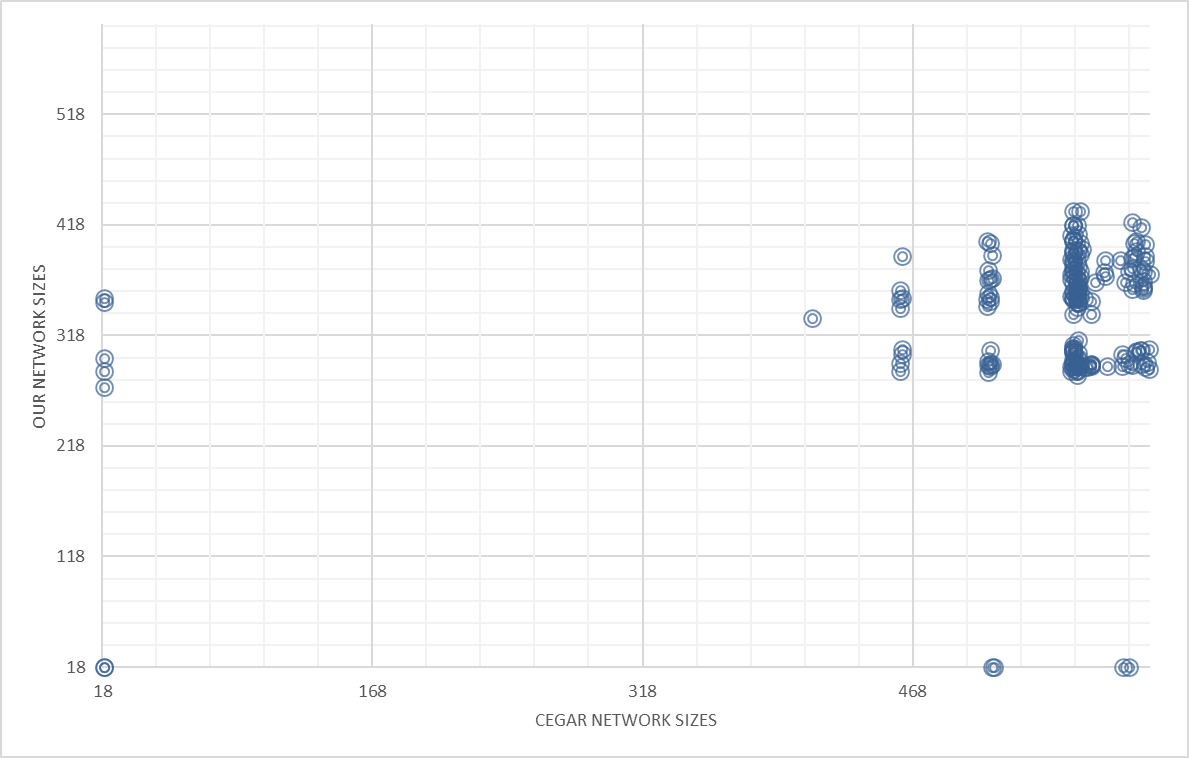
\includegraphics[scale=0.3]{figs/scatter-cegar-our-nerualsat.png}
    \caption{Scatter plot of network sizes produced by our framework vs existing
    work \cite{cegar-nn} \todo{Add diagonal line}}
    \label{f:scatter-netsizes}
    \vspace*{-1cm}
\end{wrapfigure}

For each framework, we collected the final \abs at the end of the \cegar
iterations, for which either the property can be proved to be safe, or 
the solver is able to find an actual counterexample, or the solver times out.  
Figure \ref{f:scatter-netsizes} shows a scatter plot comparing the sizes of these final \abs
obtained by our framework and by existing work \cite{cegar-nn} for each instance
in the benchmark. It is apparent from the Figure \ref{f:scatter-netsizes}, 
table \ref{t:acas-verif} and table \ref{t:acas-verif-robustness} that compared 
to the existing techniques, we are explore smaller \abs that are effective 
at proving or disproving the property in question.
This shows that using semantic information to guide the \cegar process can
effectively find more efficient abstractions than the existing technique.

Note that in our experiments, we found that the time taken by both our \cegar
approach and the existing \cegar approach \cite{cegar-nn} was more than what the
\neuralsat solver takes for the \acasxu benchmarks. However, while we would
expect the solver call times to exponentially scale with network size, the
overheads from the abstraction procedure will not scale exponentially. Thus, for
larger and larger benchmarks, being able to find smaller \abs will produce a
significant difference in times. Furthermore, we believe that a verified \abs is
useful beyond verifying a single property - it may be used for other related
queries, or may be useful as a safely deployable compressed network.
\dmcmt{Is this okay?} 

\dmcmt{Do we need the following?}
Additionally, we find that the final solver times on the \abs are actually
comparable with the times obtained on the original un-abstracted \cnc. In
general it has may observed, both by our experiments and in \cite{cegar-nn},
that the effort needed to verify a network is dependent
on more than just network size. In fact, in \cite{cegar-nn},
they are able to achieve smaller solver times on larger networks. 
While it is true that in general the worst-case performance of neural network
solvers will almost certainly remain exponential in the size of the network
\cite{reluplex}, other factors on which the performance of neural network
solvers may depend on remains an interesting direction of future work. \dmcmt{Is
this okay?}

